\documentclass[a4paper, 11pt]{extarticle}

% PDF search & cut'n'paste
\usepackage{cmap}

% Better sans-serif fonts
%\usepackage{pscyr}
\renewcommand{\rmdefault}{cmr}
\renewcommand{\sfdefault}{ftx}
\renewcommand{\ttdefault}{cmtt}

% Cyrillic support
\usepackage{mathtext}
\usepackage[T2A]{fontenc}
\DeclareSymbolFont{T2Aletters}{T2A}{cmr}{m}{it}
\usepackage[utf8]{inputenc}
\usepackage[english]{babel}

% AMS font faces
\usepackage{amsmath, amsfonts, amssymb, amsthm}

% Support for the upright and bold greek letters
\usepackage{bm}
\usepackage[Symbolsmallscale]{upgreek}
\makeatletter
        \newcommand{\bfgreek}[1]{\bm{\@nameuse{up#1}}}
\makeatother

% Detect whether PDFLaTeX is in use
\usepackage{ifpdf}

% Graphics
\ifpdf
  \usepackage[pdftex]{graphicx}
  \graphicspath{Figures/}
  \DeclareGraphicsExtensions{.png,.eps,.pdf}
\else
  \usepackage{graphicx}
\fi

\graphicspath{{Figures/}}

% Indent the first paragraph as well
\usepackage{indentfirst}

% According to GOST, sections should be called chapters in diploma
\usepackage{titlesec}

% Configure numbering in TOC section
\setcounter{tocdepth}{2}

%\titleformat{\section}[block]{\bfseries\large\sffamily\raggedright}
%        {Chapter~\Roman{section}.}{1ex}{}
%\titleformat{\subsection}[block]{\bfseries\normalsize\sffamily\raggedright}
%        {\arabic{section}.\arabic{subsection}.}{1ex}{}
%\titleformat{\subsubsection}[block]{\normalsize\sffamily\raggedright}
%        {\arabic{section}.\arabic{subsection}.\arabic{subsubsection}.}{1ex}{}

%\titlespacing*{\section}      {0pt}{3.50ex plus 1ex minus .2ex}{2.3ex plus .2ex}
%\titlespacing*{\subsection}   {0pt}{3.25ex plus 1ex minus .2ex}{1.5ex plus .2ex}
%\titlespacing*{\subsubsection}{0pt}{3.25ex plus 1ex minus .2ex}{1.5ex plus .2ex}

\usepackage[titles]{tocloft}

%\renewcommand{\cftsecpresnum}{Chapter~}
%\renewcommand{\cftsecleader}{\bfseries\cftdotfill{\cftdotsep}}
%\renewcommand{\cftsecaftersnum}{.}
%\renewcommand{\cftsubsecaftersnum}{.}

\newlength{\zyvseclen}
\settowidth{\zyvseclen}{\bfseries\cftsecpresnum\cftsecaftersnum}
\addtolength{\zyvseclen}{2mm}
\addtolength{\cftsecnumwidth}{\zyvseclen}

\renewcommand{\thesection}{\Roman{section}}
\renewcommand{\thesubsection}{\arabic{section}.\arabic{subsection}}
\renewcommand{\thesubsubsection}
        {\arabic{section}.\arabic{subsection}.\arabic{subsubsection}}

% Page numbering at the right topmost part of the page
\pagestyle{myheadings}

% Provides support for setting the spacing between lines in a document. Package
% options include singlespacing, onehalfspacing, and doublespacing.
% http://www.ctan.org/tex-archive/macros/ ... /setspace/
\usepackage{setspace}

% Alternative geometry
\usepackage[top=2cm, bottom=2cm, left=3cm, right=1cm]{geometry}

% Hyperlinks
\ifpdf
        \usepackage[pdftex]{hyperref}
\else
        \usepackage{hyperref}
\fi

\hypersetup{
        unicode=true,
        pdftitle={
        },
        pdfauthor={},
        pdfkeywords={
        },
        colorlinks,
        citecolor=black,
        filecolor=black,
        linkcolor=black,
        urlcolor=blue
}

% Fix links to floats
\usepackage[all]{hypcap}

% Add subfloats
\usepackage[font=footnotesize]{subfig}

% Nice citations [1,2,3,4] -> [1-4]
\usepackage[numbers,sort&compress]{natbib}

% [1] -> 1. in the bibliography
\makeatletter
\renewcommand\@biblabel[1]{#1.}
\makeatother

% Russian-styled figure and table captions
\usepackage[labelsep=period]{caption}

% Here we define the relationships for the counters: normaly we should
% reset the eq, figure & table counters every chapter
\makeatletter
\@addtoreset{equation}{section} % Equation counter
\@addtoreset{figure}{section} % Figure counter
\@addtoreset{table}{section} % Table counter
\makeatother

\renewcommand{\theequation}{\arabic{section}.\arabic{equation}}
\renewcommand{\thefigure}{\arabic{section}.\arabic{figure}}
\renewcommand{\thetable}{\arabic{section}.\arabic{table}}

\renewcommand{\epsilon}{\varepsilon}

\newcommand{\States}{\mathcal{S}}
\newcommand{\Actions}{\mathcal{A}}
\newcommand{\Rewards}{\mathcal{R}}
\newcommand{\TransitionProb}{\mathcal{T}}

\newcommand{\walls}[1]{\left | #1 \right |} % |smth_vertically_large|
\newcommand{\pars}[1]{\left( #1 \right)} % (smth_vertically_large)
\newcommand{\class}[1]{\left[ #1 \right]} % [smth_vertically_large]
\newcommand{\braces}[1]{\left\{ #1 \right\}} % {smth_vertically_large}
\newcommand{\len}[1]{\walls{#1}}
\newcommand{\abs}[1]{\walls{#1}}

% Package for writing pseudo-code.
\usepackage{algpseudocode}
\usepackage{algorithm}

\newtheorem{theorem}{Theorem}
\newtheorem{lemma}{Lemma}
\newtheorem{corollary}{Corollary}

% Keeps floats `in their place', preventing them from floating past a
% "\FloatBarrier" command into another section.  The floats should not move
% past every "\section".
\usepackage[section]{placeins}

% Compressed lists: compactitem etc.
\usepackage{paralist}

% Useful for individually placing figures on a separate page with
% \afterpage{\clearpage \begin{figure}[p] ... }
\usepackage{afterpage}

% Allow landscape pages for graphics, call like:
%
%       \afterpage{\clearpage
%       \begin{landscape}
%       \begin{figure}[p]
%       ...
%       \end{figure}
%       \end{landscape}
%       }
\ifpdf
        \usepackage{pdflscape}
\else
        \usepackage{lscape}
\fi

% This declaration makes TeX less fussy about line breaking. This can
% prevent overfull boxes, but may leave too much space between words.
% As this really isn't a fine art typography, we'll turn it on, so
% we won't have paragraphs which spans on the margins...
\sloppy

\begin{document}

% ------------------------------------------------------------------------------

% Title
% Title page.

\thispagestyle{empty}

\begin{center}

  \textsc{Федеральное Государственное Автономное Образовательное Учреждение}\\[0.2cm]

  \textsc{Высшего профессионального образования \\ <<Национальный исследовательский университет Высшая Школа Экономики>>}\\[0.7cm]

  \textit{Факультет компьютерных наук}\\[0.5cm]
  
  Кашин Андрей Андреевич \\ [0.5cm]

  \begin{Large}
    \textsc{\textbf{Application of Deep Neural Networks for Decision Making in First-person Shooter}}
  \end{Large}\\[1cm]

  \textsc{Выпускная квалификационная работа - МАГИСТЕРСКАЯ ДИССЕРТАЦИЯ \\
  по направлению 01.03.02 Прикладная математика и информатика \\
  Программа: Науки о данных}\\[0.7cm] 
  
  \rule{\textwidth}{0.5pt}\\[1.5cm]

\end{center}

\begin{center}
  \begin{tabular}{lr}
    Студент &
    Кашин А.А.
    \\[0.7cm]
    Научный руководитель &
    Макаров И.А.
  \end{tabular}

  \vspace{1.5cm}

  \vfill
  г. Москва, 2015

\end{center}
% ------------------------------------------------------------------------------

% Table of content
\tableofcontents
% ------------------------------------------------------------------------------

% Main section 
\begin{onehalfspacing}
    \section{Introduction}

%% Общее правило на введение - почти каждое нетривиальное утверждение должно подкрепляться релевантной, желательно актуальной ссылкой на научные источники или технические отчеты.

%% Вставь введение про видео-игры, жанр FPS и его важность в прогрессе аппаратных и программных решений для игровой индустрии (см. драфт статьи altmm).

Decision making in multiplayer first-person shooters poses many challenges for computer algorithms.
The algorithm should possess a variety of skills in order to perform successfully in the game,
for example ability to do prediction of enemy's actions, long-term planning, cooperation with other
bots.
It's very complicated to incorporate all this skills into a single hand-crafted algorithm because
it's often hard to formalize this concepts and the search space is vast.

Creating a multi-purpose first person shooter bot with reinforcement learning

Give a summary of pros and cons of this solution.

% У меня в статьях обычно это обосновается идеей создания унифицированногой модели поведения, которую разработчику не надо было бы настраивать вручную, прописывая скриптовое поведение на каждую ситуацию
% Отсюда идея обучения
% После чего нужно вставить обзор SL работ, которые занимались имитацией человека на основе логов игры
% См. публикации проекта http://www.botprize.org/publications.html

This problems lead to development of a new family of self-improving control algorithms based on machine learning techniques,
known as Reinforcement Learning algorithms.

% Описание идеи, примеры успешных приложений, 2-3 ссылки

% Следующий переход - успехи в CV и появление DRL алгоритмов, работающих с визуальными состояниями

These class of algorithms has proven to be highly successful in many game settings,
ranging from Atari games \cite{Atari} to classic board game of Go \cite{AlphaGo}.

One of the main component of the state-of-the-art reinforcement learning agents are deep neural networks that are used as function approximators for state-value function or policy function.
The area of deep learning has been rapidly developing in the latest years providing many useful
instruments that allowed agents to be trained on raw pixels in end-to-end fashion.
Application of recurrent neural networks\cite{RLRNN} and memory units (e.g. LSTMs \cite{TextGamesLSTM}) helped to tackle problems that require long-term planning.
Finally, transfer learning (CITE) and curriculum learning \cite{Curriculum} techniques allowed to reuse the same architecture to handle different tasks and also greatly stabilized training.

%% Переносим этот кусок в раздел после шутера, то есть до описания методов. Это наша мотивация и она должна идти до описания основных результатов в области

The games are a perfect testbed for evaluating this algorithms for several reasons:
\begin{itemize}
    \item Ease of getting training data. For all computer games there is already available simulated environment that allows to generate
        an infinite amount of training data and also to evaluate the policy on-line.
    \item Low cost of error. It's safe to experiment in simulated environment as opposed to training a robot in real world where it's actions can have external consequences. 
    \item Scalability. It's easy to speedup training and evaluation by horizontally scaling it across several parallel instances of the same environment.
    \item Auxiliary information for training. Using game engines give the ability to extract additional information about environment that can be used to accelerate training. CITE unreal.
\end{itemize}
%% Label 1

\section{FPS environment}
In this section we describe the FPS setup that we study in this work.
The player has control over the agent that lives in 3-dimensional environment , can perform several types of actions that influence this environment and has a goal that is dictated by the rules of the game.
As an input, agent receives 2-dimensional views of the environment from the first-person camera.

In our particular case there are 3 types of actions that agent can perform:
\begin{itemize}
    \item Movement --- moves the agent in direction of it's current orientation. This command will be processed by the environment to account for possible obstacles and physical laws that should be obeyed during movement.
    \item Aiming --- changes the orientation of agent in space, that is specified by 3-dimensional vector of angles.
    \item Shooting --- uses a weapon in direction of the agent's current orientation.
\end{itemize}

Each agent has an internal state that represents it's current amount of health points. This state can change under external effects, for example picking up health bonus or being damaged by other agent's shooting.
The agent's actions depend on it's internal state, when health points become negative, no more actions are available for the agent and it is eliminated from the environment.

%% Описать возможны режимы игры в FPS. Мы же тоже рассматриваем задачи Team DM и т.д.
The goal of the agent is to eliminate all agent's from the opposite team.

The problem can be split into several different tasks:
\begin{enumerate}
    \item Processing the visual input of the agent to infer information about surrounding world.
    \item Performing high-level movement commands, e.g. moving from point A to point B using primitive motions.
    \item Predict enemy's behaviour and use it to inform other actions.
    \item Cooperate with teammates to achieve the common goal.
    \item Evaluate the profit of collecting bonuses.
\end{enumerate}

Some of this tasks can be formulated as a reinforcement learning problems.
(Why do we think this is a good approach?)
We are going to address tasks X, Y, Z in this work.


%% We consider state-of-art methods for DRL, which were used for learning how to play ATARI games and, and aim to improve the learning rate of DRL algorithms applied in FPS environment with large number of possible actions.

We can apply both on-policy (A3C) and off-policy (DQN) methods for this task because the direct simulation is available for the agent.
%% Examples of successful application in Labyrinth and Montesuma, planning tasks (DRL blog on DM)

The agents will face exploration/exploitation dilemma in the case of bonuses collection, because this is an action that doesn't yield immediate reward, can pay off in the long run, but introduces some risks.
%% Ask Maria Bochkareva for complete list of bonuses with their descriptions

Our environment is partially observable, at any time agent sees only limited part of the vast environment. This means that it would be difficult to use model-based methods because they will need to represent high-dimensional hidden space. This means that we will use model-free methods.

%% All the text below (till the end of subsection) should be reorganized allowing reader to understand 'pro et contra' of each mentioned approach, preferably for game-like environment

The original game rewards are very sparse - they come only in the end of round which can last for 1000s of frames, and summarize the behaviour of the bot as the whole without giving any details about particular actions.
Reward shaping (CITE) methods might be used to introduce intermediate rewards and accelerate training. For example we might give a negative reward for losing health points, or give positive reward for discovering and damaging an enemy.

%% Add Gorrilla Google Project information and similar approaches to parallel RL in the multi-agent environment

The curriculum learning (CITE) methods might be used to mitigate a problem of sparse rewards and train agents on tasks that give more immediate rewards.

Another method for addressing rewards problem is an imitation learning (CITE) that allow to generate rewards based on the similarity of behaviour to some reference agent.

%%

\section{Previous work}

The reinforcement learning algorithms have been successfully applied in variety of tasks.

Talk about boom of reinforcement learning. \\
  - Atari \\
  - AlphaGo \\
  - Neural computers \\
  - Robotics \\

\subsection{Environments}

What are other related environments that are solved using RL? \\
- Atari games \\
- OpenAI Gym \\
- DeepMind Lab \\
- OpenAI Universe \\
- VizDoom \\

\subsection{Methods}
Mention methods to solve the problem: SARSA, TD-Learning, Q-learning
Value based vs Policy based (e.g. actor-critic) methods.

Deep reinforcement learning is a combination of Deep Learning and RL when we use neural networks as the function approximators in RL (e.g. to approximate value function). \\
- Why is this good? \\
- What problems does it solve? \\

6. Current approaches: \\
- DQN \\
- A3C \\
- UNREAL \\

%% If did not need them - do not mention them or put a short link in introductory part
7. Methods used inside RL agents \\
- GANs \\
- Planning networks \\
- Attention and Memory (DNC) \\

%% The rest part of the article is organized as follows. The Section 1 presents core definitions for RL and DRL algorithms. 

% The section 2 describes the experiment made in Pong game on synthetic environment and technological aspects of implementation.

%The Section 3 describes the structure of BOT representation in Unreal Engine 4 and the model of a game, in which we will test our agent. 


    \section{Reinforcement Learning}

Reinforcement learning usually solves sequential decision making problems. An RL agent interacts with an environment over time. At each time step $t$, the agent receives a state $s_t$ and selects an action $a_t$ from some action space $\mathcal{A}$, following a policy $\pi(a_t|s_t)$, which is the agent's behavior, i.e., a mapping from state $s_t$ to actions $a_t$, receives a scalar reward $r_t$, and transitions to the next state $s_{t+1}$, according to the environment dynamics, or model, for reward function $R(s,a)$ and state transition probability $P(s_{t+1}|s_t, a_t)$ respectively. In an episodic problem, this process continues until the agent reaches a terminal state and then it restarts. The return $R_t = \sum_{k=0}^{\infty} \gamma^k r_{t+k}$ is the discounted, accumulated reward with the discount factor $\gamma \in (0,1]$. The agent aims to maximize the expectation of such long term return from each state.     

A value function is a prediction of the expected, accumulative, discounted, future reward, measuring how good is each state, or state-action pair. The action value $Q^{\pi}(s, a) = E[R_t | s_t = s, a_t = a]$ is the expected return for selecting action $a$ in state $s$ and then following policy $\pi$. An optimal action value function $Q^{*}(s, a)$ is the maximum action value achievable by any policy for state $s$ and action $a$. We can define state value $V^{\pi}(s)$ and optimal state value $V^{*}(s)$ similarly.

Temporal difference (TD) learning is a central idea in RL. It learns value function $V(s)$ directly from experience with TD error, with bootstrapping, in a model-free, online, and fully incremental way.  The update rule is $V(s_t) \leftarrow V(s_t) + \alpha [r_t + \gamma V(s_{t+1}) - V(s_t)]$, where $\alpha$ is a learning rate, and $r_t + \gamma V(s_{t+1}) - V(s_t)$ is called TD error. Similarly, Q-learning learns action value function, with the update rule, $Q(s_t, a_t) \leftarrow Q(s_t, a_t) + \alpha [r + \gamma \max_{a_{t+1}}Q(s_{t+1}, a_{t+1}) - Q(s_t,a_t)]$. Q-learning is an off-policy control method. In contrast, SARSA, representing state, action, reward, (next) state, (next) action, is an on-policy control method, with the update rule, $Q(s_t, a_t) \leftarrow Q(s_t, a_t) + \alpha [r + \gamma Q(s_{t+1}, a_{t+1}) - Q(s_t,a_t)]$. SARSA refines the policy greedily with respect to action values. TD-learning, Q-learning and SARSA converge under certain conditions. From optimal action value function, we can derive an optimal policy. 

The above algorithms are referred to as TD(0) and Q(0), with one-step return. We have multi-step return variants or Monte-Carlo approach in the forward view. The eligibility trace from the backward view provides an online, incremental implementation, resulting in TD($\lambda$) and Q($\lambda$) algorithms, where $\lambda \in[0,1]$. When $\lambda = 1$, it is the same as a Monte Carlo approach. 

We discuss the tabular cases above, where a value function or a policy is stored in a tabular form. Function approximation is a way for generalization when the state and/or action spaces are large or continuous. Linear function approximation used to be a popular choice, esp. before the work of Deep Q-Network~\citep{Atari}.

%For TD($\lambda$), the update rule follows, $\delta_t \leftarrow r_t + \gamma V(s_{t+1}; \theta) - \gamma V(s_t; \theta), e_t \leftarrow \gamma \lambda e_{t-1} \nabla_{\theta} + V(s_t; \theta), \theta_t \leftarrow \theta_{t-1} + \alpha \lambda e_t$.

In contrast to value-based methods like TD learning and Q-learning, policy-based methods optimize the policy $\pi(a|s; \theta)$ (with function approximation) directly, and update the parameters $\theta$ by gradient ascent on $E[R_t]$. REINFORCE is a policy gradient method, updating $\theta$ in the direction of $\nabla_{\theta} \log \pi(a_t|s_t; \theta) R_t$. Usually a baseline $b_t(s_t)$ is subtracted from the return to reduce the variance of gradient estimate, yet keeping its unbiasedness, to yield the gradient direction $\nabla_{\theta} \log \pi(a_t|s_t; \theta) (R_t - b_t(s_t))$. Using $V(s_t)$ as the baseline $b_t(s_t)$, we have the advantage function $A(a_t, s_t) = Q(a_t, s_t) - V(s_t)$, since $R_t$ is an estimate of $Q(a_t, s_t)$. In actor-critic algorithms, the critic updates action-value function parameters, and the actor updates policy parameters, in the direction suggested by the critic.

We obtain deep reinforcement learning (deep RL) methods when we use deep neural networks to approximate any of the following component of reinforcement learning: value function, $V(s; \theta)$ or $Q(s,a; \theta)$, policy $\pi(a|s; \theta)$, and model (state transition and reward). Here, the parameters $\theta$ are the weights in deep neural networks. When we use "shallow" models, like linear function, decision trees, tile coding and so on as the function approximator, we obtain "shallow" RL, and the parameters $\theta$ are the weight parameters in these models. Note, a shallow model, e.g., decision trees, may be non-linear. The distinct difference between deep RL and "shallow" RL is what function approximator is used. This is similar to the difference between deep learning and "shallow" learning. We usually utilize stochastic gradient descent to update weight parameters in deep RL. When off-policy, function approximation, in particular, non-linear function approximation, and bootstrapping are combined together, instability and divergence may occur~\citep{TDWithApproximator}. However, recent work like Deep Q-Network~\citep{Atari} and AlphaGo~\citep{AlphaGo} stabilized the learning and achieved outstanding results.

We explain some terms in RL parlance. The prediction problem, or policy evaluation, is to compute the state or action value function for a policy. The control problem is to find the optimal policy. Planning constructs a value function or a policy with a model. On-policy methods evaluate or improve the behavioural policy, e.g., SARSA fits the action-value function to the current policy, i.e., SARSA evaluates the policy based on samples from the same policy, then refines the policy greedily with respect to action values. In off-policy methods, an agent learns an optimal value function/policy, maybe following an unrelated behavioural policy, e.g., Q-learning attempts to find action values for the optimal policy directly, not necessarily fitting to the policy generating the data, i.e., the policy Q-learning obtains is usually different from the policy that generates the samples.  The notion of on-policy and off-policy can be understood as same-policy and different-policy.The exploration-exploitation dilemma is about the agent needs to exploit the currently best action to obtain rewards, yet it has to explore the environment to find better actions.  In model-free methods, the agent learns with trail-and-error from experience explicitly; the model (state transition function) is not known or learned from experience. RL methods that use models are model-based methods. In online mode, training algorithms are executed on data acquired in sequence. In batch mode, models are trained on the entire data set. With bootstrapping, an estimate of state or action value is updated from subsequent estimates.

    \section{Frameworks}

General introduction to NN training and modern frameworks, tell about
TensorFlow, PyTorch, Caffe. How they support different devices, and how
this becomes increasingly important with the Moore's Law. Mention that this
is an important area of research, as it will yield big performance gains.

    \section{Environments}

% Section about environments and their performance
Environments - describe why simulated environments are used, what kind of
tasks they simulate, how they range in Accuracy, Performance, Complexity,
Usability.

In this section we will describe:
- What is the environment from RL perspective (state transition function, rewards).

Reinforcement learning algorithms usually operate in the context of the specific
environment that is characterized by it's \emph{state space} $\States$,
\emph{action space} $\Actions$, \emph{transition dynamics} $\TransitionProb(s, a, s')$ and
\emph{rewards distribution} $\Rewards(s)$.
When the agent interacts with the environment, it observes some part of the state $o(s)$,
and performs an action $a$ from the action space. This causes the environment to transition to
next state $s'$ with probability $\TransitionProb(s, a, s')$ and also gives agent a reward sampled
from $\Rewards(s')$.

When $o(s) = s$, i.e. $o(\cdot)$ is an identity function, the environment is said to be
\emph{fully observable}. Otherwise, it's \emph{partially observable}. The theory of reinforcement
learning deals with both cases, yet the second one is considered to be much more difficult.

Another important classification of environments arises from the type of the action space,
that can be either discrete or continuous. For some of the algorithms this
distinction is critical, for example vanilla Q-learning methods become infeasible in
continuous action space, as it becomes difficult to perform $max$ operator in this space.
There are some works that aim to overcome this issue \cite{NAF}.
Policy gradient methods are agnostic to the type of the action space, as long as there is
a proper reparametresation in terms of some convenient distribution (e.g. Normal).

This definition of the environment allows wide range of virtual and real-world systems to be
represented as an instance of this model. This, as a consequence, allows solving tasks of policy
estimation and optimal control for this systems.

An example of the virtual discrete environment that is widely used as a benchmark for
optimal control reinforcement learning algorithms is Arcade Learning Environment \cite{ALE},
that introduced programmatic access to 47 classic video games from Atari 2600 simulator.
Each game corresponds to a separate environment with it's own mechanics and rewards system,
including a highly visual input space. The first reinforcement learning methods that showed
super-human results on subset of this environments was a DQN \cite{DQN} algorithm.
Some of the tasks from this benchmark like Montezuma Revenge are still posing a major
challenge to the most of current algorithms.

Another family of environments that are more connected with real-world continuous control
problems like robotics are physics simulation engines. One notable example from this family
that is considered as a benchmark for continuous control algorithms is Mujoco \cite{Mujoco}.
This physics engine allows fast and high-fidelity simulation of dynamic physical systems
like multi-joint robotic arm control. The framework comes with the set of tools for
building and interacting.

It's imporant to realize, that the same environment allows different observation types -
when algorithm interacts with physics engine, it might operate on physical parameters of the
system (coordinates, velocities, accelerations) or on the video stream of the environment from
multiple cameras as it would be in real physical system. As expected, solving the control
tasks in the environment is usually much simpler from the core system parameters rather
then from the raw pixel observations.

The environments presented above are the examples with fixed environment dynamics.
This is not always true, and the important example of the environments with parameterized
transition dynamics are two-player board games. In this case, the opponent greatly influences
the behaviour of the environment. On of the first successes of application of reinforcement
learning was in the Backgammon board game \cite{TDGammon} in 1994.
Recent success in this area is the compute program AlphaGo \cite{AlphaGo} that defeated
world champion in the ancient game of Go.

- What are the examples of simulated environments (ALE, Mujoco, StarCraft, VizDoom).
- tell more about FPS environments, Dota2, why are those hard? Give the Rock-Paper-Scissors
analogy that shows that determenistic policy is not a Nash-equillibria of this game.

Simulated environments game invaluable boost to the reasearch community by providing a
safe and data-rich controllable testbed for the algorithms. Let's address each point:
\begin{itemize}
    \item Simulated environments can produce unlimited amount of data, that is so important
    for training both neural networks and reinforcement learning algorithms. In contrast to
    supervised learning where one dataset with labels is enough for training any algorithm,
    in on-policy reinforcement learning the data should come from the distribution that is
    dependant on the algorithm itself, meaning that dataset should be always collected on-line
    during the performance of the algorithm.

    \item The learning algorithm usually has no explicit goal to ensure that it's actions are
    safe for the environment, and includes a fair amount of random exploration on the early
    stages of training, which might lead to destructive behaviour when applied in real-world.
    This is especially important in areas like robotics or automated control of physical systems
    like datacenter \cite{DrData}. The simulated environment doesn't suffer from this problem,
    as mistakes can not lead to catastrophic consequences.

    \item It's often very hard to get the algorithm off the ground on a complicated task,
    and the usual approach is to build complexity gradually, for example by starting from the
    simplified feature/action space, or solving sub-goals of the bigger task in curriculum
    learning \cite{Curriculum}. This is easily achivable with flexible frameworks like
    DMLab \cite{DMLab} that allow building custom levels and expose engine information to
    the algorithm.
\end{itemize}

- How simulated environments are commonly implemented, and what implication this brings?
(limited accuracy, limited speed, limited diversity (in case of opponents in board games))

Simulated environments are usually implemented with several requirements in mind:
% Actually, I need to negate this statements. It's rather the problems of the current environments,
% something like the iron triangle, you can't have all of them.
\begin{itemize}
    \item Speed --- the environment should be able to generate big amounts of data to
    feed the training procedure. That's why most engines are implemented in low-level
    languages like C or C++.

    \item Accuracy --- for physical simulators it's particularly important to accurately reflect the
    laws of physics, as the trained algorithms are expected to transfer well to the real world,
    hopefully with minimal amount of effort.

    \item Diversity --- current learning algorithms are very prone to overfitting, meaning that
    if the environment during the training introduced some bias, for example, same color of
    walls in the maze, or same opponent in the board game, the algorithm is likely to overfit
    to this specific setting, and won't generalize well to other setting.
\end{itemize}

- Other notable progress in environments development: DeepMind Lab, VizDoom, StarCraft 2.

- How this work addresses is connected to different environments: we build an adaptive algorithm,
that can take into account the speed of the environment.

In this work we explore the architecture that can work well in slow environments by decoupling
the learning process and the interaction with environment to allow them to happen in parallel,
without blocking each other.

- Tell more about environments used in this work: VizDoom.

%\section{FPS environment}
In this section we describe the FPS setup that we study in this work.
The player has control over the agent that lives in 3-dimensional environment, can perform several types of actions that influence this environment and has a goal that is dictated by the rules of the game.
As an input, agent receives 2-dimensional views of the environment from the first-person camera.

In our particular case there are 3 types of actions that agent can perform:
\begin{itemize}
    \item Movement --- moves the agent in the direction of specified 3-d vector. This command will be processed by the environment to account for possible obstacles and physical laws that should be obeyed during movement.
    \item Aiming --- changes the orientation of agent in space, that is specified by 3-dimensional vector of angles.
    \item Shooting --- uses a weapon in direction of the agent's current orientation.
\end{itemize}

Each agent has an internal state that represents it's current amount of health points. This state can change under external effects, for example picking up health bonus or being damaged by other agent's shooting.
The agent's actions depend on it's internal state, when health points become negative, no more actions are available for the agent and it is eliminated from the environment.

%% Описать возможны режимы игры в FPS. Мы же тоже рассматриваем задачи Team DM и т.д.
The goal of the agent is to eliminate all agent's from the opposite team.

The FPS problem can be split into several different tasks:
\begin{enumerate}
    \item Navigation
    \item Combat
\end{enumerate}

Some of this tasks can be formulated as a reinforcement learning problems.
% Add links about previous approaches to each of the tasks described with summary of the
% achieved results on them. What was successful? What needs to be addressed in the future?
We are going to address tasks X, Y, Z in this work.

%% We consider state-of-art methods for DRL, which were used for learning how to play ATARI games and, and aim to improve the learning rate of DRL algorithms applied in FPS environment with large number of possible actions.

We can apply both on-policy (A3C) and off-policy (DQN) methods for this task because the direct simulation is available for the agent.
%% Examples of successful application in Labyrinth and Montezuma, planning tasks (DRL blog on DM)

The agents will face exploration/exploitation dilemma in the case of bonuses collection, because this is an action that doesn't yield immediate reward, can pay off in the long run, but introduces some risks.
%% Ask Maria Bochkareva for complete list of bonuses with their descriptions

% This should be somewhere near environment description.
Our environment is partially observable, at any time agent sees only limited part of the vast environment. This means that it would be difficult to use model-based methods because they will need to represent high-dimensional hidden space. This means that we will use model-free methods.

Our goal is to create an agent with the same set of inputs and actions as the human-player.

%% All the text below (till the end of subsection) should be reorganized allowing reader to understand 'pro et contra' of each mentioned approach, preferably for game-like environment

The original game rewards are very sparse - they come only in the end of round which can last for 1000s of frames, and summarize the behaviour of the bot as the whole without giving any details about particular actions.
Reward shaping \cite{RewardShaping} methods might be used to introduce intermediate rewards and accelerate training. For example we might give a negative reward for losing health points, or give positive reward for discovering and damaging an enemy.
Agent might also benefit from intrinsic motivation signals \cite{IntrinsicMotivation}.

%% Add Gorilla Google Project information and similar approaches to parallel RL in the multi-agent environment

The curriculum learning (CITE) methods might be used to mitigate a problem of sparse rewards and train agents on tasks that give more immediate rewards.

Another method for addressing rewards problem is an imitation learning (CITE) that allow to generate rewards based on the similarity of behaviour to some reference agent.


%\section{Pong}

In this section we describe application of Deep RL methods to a game of Pong implemented inside Unreal Engine 4 (UE4) environment.
Unreal Engine 4 is a suite of integrated tools for game developers to design and build games, simulations, and visualizations.

The main goals of this work is to prove that RL applied inside UE4 it's technically feasible solution: it's should be possible to efficiently train and apply model built with modern machine learning framework (in our case TensorFlow).

We achieve this by patching a plugin to support Python scripting inside UE4, implementing C++ module for capturing game screenshots, and creating TensorFlow-based Python controller for the player paddle.

\subsection{Environment}

We use physics based UE4 implementation of classical \href{https://en.wikipedia.org/wiki/Pong}{Pong} environment. 
\begin{figure}[h!]
\caption{Pong Screenshot}
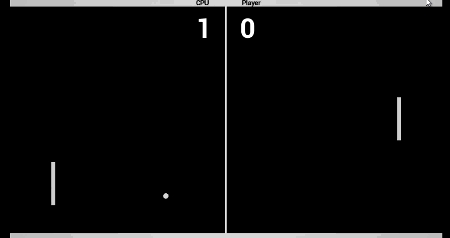
\includegraphics[width=\textwidth]{PongPhys}
\end{figure}

This screenshot from the environment shows main elements of the game:
\begin{enumerate}
    \item Paddles ---
        Every player controls a solid rectangle called paddle that can reflect the ball.
    \item Ball ---
        The ball is a rigid body that moves with a constant speed and reflects from the walls and paddles.
    \item Walls ---
        The walls are present on the top and on the bottom of the screen.
    \item Goals ---
        The left and right sides of the screen represent goals. In order to score a point, the player needs to hit the opposite goal with the ball.
    \item Scores ---
        The top part of the screen shows two numbers that are equal to the number of points each player have scored.
\end{enumerate}

The purpose of the game is to maximize the difference between your score and opponent score.

The human player uses raw pixels (screenshots) as an input during play, and outputs three types of actions using the keyboard:
\begin{itemize}
    \item Key up --- move paddle up
    \item Key down --- move paddle down
    \item Idle --- paddle stays at the same place
\end{itemize}

The game comes with the built-in AI controller that gets high-level features such as position and speed of the ball, position of his and opponent paddle as an input,
and uses rule-based approach to control the paddle.

\subsection{Python Scripting}

In Unreal Engine 4, the standard way to implement game logic is through writing C++ modules or using internal visual scripting language called Blueprints.
The C++ approach is more powerful and is used to implement core game logic and reusable modules, though in many cases it's overly verbose, and doesn't allow to quickly iterate on the solution due to slow compilation speeds.
On the other hand, blueprints are simple to create and understand, allow faster development cycles, yet not expressible enough in many cases.

When it comes to the modern machine learning engines, they are usually written in C++, while the public API that they provide comes in form of Python bindings.
While in principle it's possible to use TensorFlow C++ API, this approach limits the reuse of openly available RL algorithms implementations in Python, and slows down the research process due to the nature of the C++ language.

Due to all this reasons we looked into alternative languages support for UE4 and identified two candidates: Python and Lua.
Both languages are supported through third-party plugins available on GitHub, \href{https://github.com/facebook/UETorch}{UETorch} for Lua and \href{https://github.com/20tab/UnrealEnginePython}{UnrealEnginePython} for Python.

As the authors were more familiar with Python and TensorFlow, it was chosen as the primary language.
During this work, the original plugin was extended to support Python-based controllers in UE4.

The plugin allows users to write Python scripts that interact with UE4 engine by being able to access and mutate the internal state of the game.
This can be used to obtain current position of the ball and paddle, and giving the commands to move the paddle.

\subsection{RL Model}

We implement bot controller using TensorFlow machine learning framework \cite{tensorflow2015-whitepaper} to utilize GPU and multi-core CPU resources.
We use Deep Q-Network (DQN) \cite{mnih-dqn-2015} learning algorithm to train and control the bot.
The reward of +1 is given to the bot when it scores a point, and -1 when the opponent scores a point.

The bot is trained with fixed FPS 32. The screenshots are binarized and rescaled to resolution 80x80.

\subsection{Results}

We've built a Deep RL based controller that outperforms the standard rule-based bot, while using raw pixels as an input.
The training usually takes 6 hours on GPU and it takes 10 million iterations to beat the built-in scripted bot.

The code implementation is available on \href{https://github.com/akashin/HSE_AI_Labs/tree/master/Lab_4}{GitHub}.

    \section{HardwareAndTraining}

% Section about hardware and utilization

- GPU vs CPU for training, motivation, comparison of performance, support
  from different frameworks, cost, restrictions, dependence on the size of
  the network. Sampling on CPU is fine, but parallelism is very bad.
  Mention last paper by Facebook about ImageNet. Mention the paper Learning
  to play in a day.

In this section we describe:
- How training is usually performed for RL algorithms: typical loop of samples collection
and training. Difference between off-policy and on-policy algorithms.

Usually, the reinforcement learning algorithms training consists of the following components

\begin{itemize}
    \item Acting in the environment. At this step, the agent observes the current state of the
    environment and makes the decision which action to take. This usually involves making one
    forward pass in the neural network that represents the policy of the agent.

    \item Sampling an observation from the environment. At this step the underlying simulator consumes
    the action provided by the agent and performs transition to the next state, that might also
    yield some reward visible to the agent. This step involves the simulator performing computations
    with regards to the environment transition dynamics, and can be performed on CPU or on GPU for
    the visuallty demanding environments.

    \item Collecting the state transition to the dataset used to train the agent. At this step
    the agent usually records a tuple $(s, a, r, s')$ that represents one transition and
    consists of previous state, action, reward, and the resulting state.

    \item Using the collected data to improve the policy. This step uses the data that was collected
    during the interaction with the environment to update parameters of the policy in such way that
    it improves the average reward received by agent. Usually this step resembles solving a
    supervised learning problem.
\end{itemize}

Depending whether the learning algorithm is on-policy or off-policy, the fate of the collected
dataset will depend. For off-policy learning, the dataset might be kept between different updates
to the policy. In on-policy learning, dataset is usually discarded after any big change to the
policy, as it greatly changes the distribution of data and introduces bias to the training
procedure.

Different training components might benefit from different hardware type. The acting and sampling
from the environment requires low-latency computation to deliver good throughput. This is well
suited for fast CPUs or GPUs, though the later tend to be underutilized on such workloads.
For most training regimes there is no strict requirement that all samples are comming from the
same environment, which allows a simple data-parallel training scheme in which agent is interacting
with multiple copies of environment running in parallel. This allows to achieve the same data
throughput without the need for high-performance sampler. This scheme might be more memory intensive
though, and also requires additional synchronization mechanisms during collection of data
and acting in the environments using the same model.

When it comes to the training step, it is usually perceived as a supervised-learning task
optimized using stochastic gradient descent on the subset of currently collected transitions.
As the most popular learning models for RL nowadays are neural networks, this procedure
benefits from hardware that is tailored for running deep neural networks, for example GPUs
or TPUs \cite{TPU}. One caveat though is that the models required for most of RL tasks today
are considered small and shallow (millions of parameters) compared to those, used on
computer vision or machine translation tasks (billions of parameters). This limits the benefits
from model parallelism during training.

Another compelling option is distributed training, in which multiple possibly different compute
nodes are involved, executing one or several learning components. The example of such architecture
for reinforcement learning is GORILA \cite{GORILA} which is a general way to perform off-policy
Q-Learning. This architecture decomposes training into three components:
\begin{itemize}
    \item Actor - instance of environment and q-network that interacts with this environment.
        Actor collects training experience and sends it to global experience replay memory.

    \item Learner - instance of q-network that processes experience from replay memory and
        generates updates to policy (stochastic gradients) that are sent to parameter servers.

    \item Parameter server - holds part of the parameters of the policy/q-network. This component
        receives gradients from learners and applies them to the current model parameters.
\end{itemize}

This architecture has very good scalability properties, allowing to spawn actors and learners
independently, based on the properties of the problem at hand. It also supports heterogenous
components - learners might use GPUs and actors and parameter servers might run entirely on CPU.
One of the limitations of this architecture is that it's not suitable for on-policy learning,
as the delay between experience being produced and used for training is unbounded, and there
are no guarantees on freshness of parameters used by actors.

When it comes to on-policy learning, the tight feedback loop between actor and learner becomes
extremely important. One of the architectures that implements this is called A3C \cite{A3C}, that
stands for asynchronous advantage actor-critic. This algorithm implements actor-critic policy
gradient method, that is trained solely on CPU. All training components are located on the
single machine and share policy parameters in a shared memory. The actor and the learner are
bundled together into actor-learner component, and experience produced by the actor is immediatly
consumed by the corresponding learner to compute a gradient update to the shared parameters.
Multiple actor-learners are running at the same time independently, and their number usually
depends on the number of CPU cores on the machine. It's important to note, that this architecture
it still slighly off-policy, as the learners are contributing the gradients to the shared parameters
that does not always correspond to the parameters that they were acting with, though this amount
of staleness does not visiably influence the stability of the algorithm at this scale.

The vanilla A3C was running solely on CPU cores without any hint on GPU usage, but there are
several follow up works that showed how to efficiently utilize GPUs for this task. The general
motive is to take advantage of GPUs ability to process big batches of data in parallel.
This approach is used in GA3C \cite{GA3C}, that proposes to perform all neural network computations
(actions and training) on GPU in a batched manner. This is achieved through introducing a system
of queues for acting and training requests. When the actor needs to decide on the action it
posts a request to the \emph{prediction queue}, that is periodically processed by predictor threads,
that in turn perform this predictions on GPU and return the result to requester.
The actors send the observed transitions to the \emph{training queue} that is also periodically
processed by the trainer threads that perform the actual update of the model on the GPU.

One aspect of training procedure that is often disregarded is the amount of RAM allocated during
training. The algorithms like DQN usually require huge amount of memory to operate store the
replay table. For example for Atari games, the replay table in DQN \cite{DQN} paper stores
last 1 million transitions, which is around 50GB - something that is only common on big server
machines.

When using stochastic gradient descent, one important parameter that is directly connected both
with training speed and resource efficiency of the training procedure is the size of batch of
samples that is used to make compute a gradient for one step. As a rule, the bigger batch size
is, the more efficient it is to perform the computation of massively parallel hardware like
GPUs and TPUs, because this hardware benefits from homogenuous computations and model parameters
sharing across several computations. From another perspective, batch size influences the noisiness
of the gradient estimate that is used during update, and this in turn correlates with the
convergence speed of the model. In particular, high variance gradients are a common reason of
divergence of policy-gradient reinforcement learning methods. Seeing the benefits of large batch
size, one might ask why aren't we making batch sizes as big as possible? There are at least two
reasons why this is not always wise idea: first, it increases the computation cost of the
algorithm, which actually was a motivator for developing stochastic gradient descent. Second
reason, is the fact that after some threshold, adding more samples to batch would not contribute
much to the quality of obtained gradients. This is a consequence of well known central limit
theorem that in particular tells that the variance of the Monte-Carlo estimate shrinks by a factor
of $1/\sqrt{N}$ where $N$ is the sample size.
Another parameter that is somewhat connected to the batch size is the learning rate. In general,
you want to keep learning rate small when you're not sure about the gradient updates, and increase
it when you believe that the gradients give a good estimate of the direction of the optimal point.
When the batch size is large, one can be more sure about the quality of gradient and increase the
learning rate. Great example of this approach is shown in the paper that claims to train an image
classifier for ImageNet dataset in one hour with batch size of 8196 images on cluster of GPUs
\cite{1hour_imagenet}, by also introducing the learning rate scaling procedure. This result also
achieves 90\% scaling efficiency when moving from 8 GPUs to 256 GPUs.

The question of choosing good batch size for reinforcement learning algorithms didn't receive
much attention in the literature so far. The nature of optimization procedure introduces additional
challenges here - the training target is usually moving, the distribution of training data changes,
the quick feedback loop between the trained model and acting in environment is important.

In this work we are looking at the effect of different batch sizes and learning rates on the
learning algorithm as well as hardware efficiency when using GPU. This is motivated by the fact
that many of the existing algorithms are not producing non-hardware friendly workloads, and this
leads to poor utilization. One such example is the DQN algorithm, that in basic implementation
leads to 30\% of GPU utilization because it interleaves cheap prediction steps and expensive
training steps in the same thread. The A3C algorithm also didn't take advantage of specialized
hardware until the recent work on GA3C.

- Graphs about utilization of hardware with
different batch size and train frequency in DQN here.

    \section{Efficient architecture}

For building an efficient training architecture, we start by answering the following questions:

\begin{itemize}
    \item What is the family of algorithms that should be supported by this architecture? --- In
    this paper we are aiming to provide a training architecture that will cover model-free
    off-policy and on-policy algorithms with bounded staleness of samples.

    \item What hardware will be used to run the algorithm? --- We consider hybrid CPU/GPU system,
    as it's currently the most widely used platform for training neural networks, and also because
    it provides a good balance between sampling and training performance.

    \item What are the bottlenecks that prevent current algorithms to perform well? --- Most of the
    current algorithms introduce sequential dependency between acting and training procedure, that
    is absolutely unnecessary and prevents from fully utilizing a hardware and also leads to the
    slowdown when there is a skew in components performance.
\end{itemize}

We end up with the architecture that consists of the following components:
\begin{itemize}
    \item Actor --- interacts with the environment, by acting and collection the experience. To
        make actions. Uses a separate model replica that is periodically synced with the master replica.
        Runs on CPU, as it doesn't require parallelism or low-latency. Can be scaled up to several
        instances to address slow environment problem.

    \item Trainer --- collects the experience produced by actors and decides which samples will be
        used by learner to train the model. This might include using an internal experience replay
        table or just filtering old samples and forwarding them to the learner.

    \item Learner --- consumes samples provided by trainer to compute gradients and update the
        master model. Runs on GPU, as it needs to perform heavy batch computations.
\end{itemize}

\begin{figure}[h!]
\caption{Training architecture}
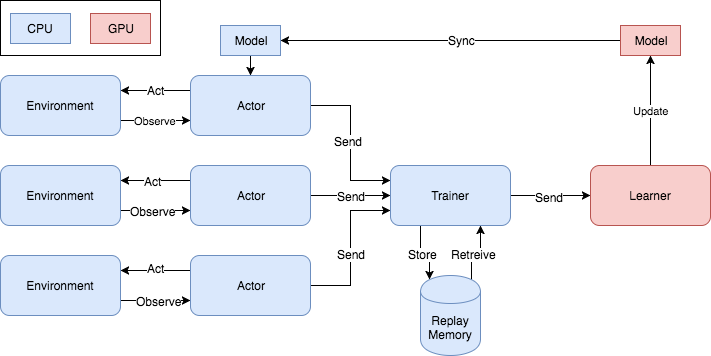
\includegraphics[width=\textwidth]{architecture}
\end{figure}

\begin{algorithm}
    \caption{Actor thread}\label{actor}
    \begin{algorithmic}[1]
        \State $env \gets MakeEnv(seed)$
        \State $state \gets env.Start()$
        \State $T \gets 0$
        \While{TrainingNotDone}
            \If{$T \mod F_{sync} = 0$}
                \State $model \gets SyncModel()$
            \EndIf
            \State $action \gets model.Predict(state)$
            \State $nextState, reward \gets env.Act(action)$
            \State $actorQueue.Enqueue(state, action, reward, nextState)$
            \State $state \gets nextState$
            \State $T \gets T + 1$
        \EndWhile
    \end{algorithmic}
\end{algorithm}

\begin{algorithm}
    \caption{Trainer thread}\label{trainer}
    \begin{algorithmic}[1]
        \While{TrainingNotDone}
            \State $states, actions, rewards, nextStates \gets actorQueue.Dequeue()$
            \State $StoreExperience(states, actions, rewards, nextStates)$
            \State $learnerQueue.Enqueue(SampleExperience(batchSize))$
        \EndWhile
    \end{algorithmic}
\end{algorithm}

\begin{algorithm}
    \caption{Learner thread}\label{learner}
    \begin{algorithmic}[1]
        \For{$T \gets 0, T_{max}$}
            \State $batch \gets learnerQueue.Dequeue()$
            \State $Train(batch)$
        \EndFor
    \end{algorithmic}
\end{algorithm}

- Description of more efficient architecture, and questions that we need to
  answer to build it. Compare with PAAC, GA3C, tell when one is better then
  the other and vice versa.

In this section we describe:
- Tell that this is our new ideas.

- Tell how it looks like. Simple description of the process in terms of multiple CPU and 1 GPU.

- Give a code for actor, trainer and learner.

- Tell how this compares to other architectures, in what regimes it should operate better then
the other algorithms.

- Tell about resulting GPU utilization and time spent in different modes of operation.

- Tell about existing bottlenecks, what will be the limiting factor depending on the env speed,
training speed, network size.

- Tell how this is applicable to DQN and ACER (and any algorithm with experience replay, or
slightly off-policy data tolerance).

    \section{Benchmarking}

- Comparison of DQN, DecoupledDQN on VizDoom.
- Comparison of DQN, DecoupledDQN on Atari, at least few games. Hopefully as much as possible.

In this section we show:
- Description of the evaluation setup, how long the models trained, which hardware was used,
which networks were used. Any specifics of the traning procedure. Sizes of the replay tables,
learning rates.

- Graphs of DQN, DecoupledDQN performance on 5 VizDoom Gym levels.

- Graphs of DQN, DecoupledDQN performance on 3 Atari games.

- Explanation what is on the graph, how we made the measurements robust to the noise (choosing top 5
from several random seeds).

- Explanation why the algorithms perform as they do. Study on how hyperparameters influence
the performance both in terms of training speed and efficiency.

- How the methods perform in terms of wall time/sample efficiency.

    \section{Conclusion}

Here we give conclusion.
\end{onehalfspacing}
% ------------------------------------------------------------------------------

% References
\phantomsection
\renewcommand{\refname}{References}
\addcontentsline{toc}{section}{References}

\bibliographystyle{gost780u}
\bibliography{Bibliography}
% ------------------------------------------------------------------------------

\end{document}
